\chapter{Topological Classification of motional modes in Rydberg atom arrays}
The possibility of trapping atoms in optical tweezers and arranging them in arbitrary geometries has inspired the investigation of various topological properties in such arrays. One of the targets of such investigations has been the motional modes of the atoms in the array. As the atoms move in the harmonic oscillator potential of the tweezer, the interaction between atoms, which are distance dependent, also change. This leads to a coupling between the motional modes of the atoms. In this work the atoms will occupy Rydberg states leading to dipole-dipole or van der Waals interactions. There are two regimes of interest, which behave in a different way. If the trap depth is much larger than the interaction, the generation of additional motional excitations is suppressed, and only hopping of motional excitations between sites takes place. Thus topological classification can exploit the single particle property of the dynamics. In the complementary regime the excitation number is not conserved and one has to deploy a bosonic formalism for the topological classification, via the Bogoliubov de Gennes (BdG) picture, discussed in the previous chapter. In the next section it is briefly discussed why both regimes can be implemented in Rydberg atom arrays.

\section{Parameter regimes}
Important for the presence or absence of motional excitation number conservation is the ratio of interaction strength $V$ to trap depth $\omega$. The lifetime of the Rydberg states $T$, however, sets a lower bound on the interaction strength, as the dynamics induced by the interaction has to be faster than the lifetime of the Rydberg state, in order to be observed. For the regime, in which the motional excitation number is conserved, the trap depth has to be much larger than the interaction which in turn has to be much larger than this lower bound. In the following I will discuss the relevant energy scales and show that both regimes can be implemented in Rydberg atom arrays.

The lifetimes for conventional Rydberg states can reach up to several hundred $\mu$s. For Circular Rydberg states the lifetimes can reach even a few ms. In both cases the trap depth ($\omega$) can have values of a few MHz \cite{wilsonTrappingAlkalineEarth2022,holzlLongLivedCircularRydberg2024}. Correspondingly the lower bound for the interaction strength is located at $V>>1/T\sim1\,$kHz. With the trap depth being in the MHz range, the conditions of conserved motional excitation number can be easily met, as the interactions between Rydberg atoms can be tuned in wide range from kHz to GHz. Due to this large flexibility in the interaction strength, also the complementary regime of non-conserved motional excitation number can be realized. In the following I will derive the effective Hamiltonian for the motional modes.


\section{Model}\label{sec:model derivation}
For the topological analysis a model will be used, that only takes motional degrees of freedom into account. This can be achieved by assuming that all atoms are in the same internal state, and the interaction doesn't couple different states. The interaction that results by this is a van der Waals interaction for atoms in Rydberg states or a dipole-dipole interaction if the atoms are dressed with an external field. I will keep the form of the interaction general in the following derivation. The system consists of $N$ atoms, which are trapped in optical tweezers with centers $\{\mathbf{R}_l\}_{l\in\{1,\dots,N\}}$. The Hamiltonian that describes the model consists of the harmonic trap potential part $\mathcal{H}_0$ and an interaction part $\mathcal{H}_I$, that depends on the position of the atoms.
\begin{align*}
    \mathcal{H} &= \mathcal{H}_0 + \mathcal{H}_I(\{{\mathbf{R}}_l\})\\
    \text{with}\quad\mathcal{H}_I(\{{\mathbf{R}}_l\}) &= \half \,\sum_{i,j}V_{i,j}(\{{\mathbf{R}}_l\})\,n_i n_j\\
    \text{where}\quad V_{i,j}(\{{\mathbf{R}}_l\})&=V({\mathbf{R}}_i,{\mathbf{R}}_j)
\end{align*}
The operators $n_i$ are the projectors on the internal state of the $i$th atom. As all atoms are assumed to be in the same internal state, the $n_i$ become redundant and can be dropped. The interaction Hamiltonian then reads

\begin{align*}
    \mathcal{H}_I(\{{\mathbf{R}}_l\}) = \sum_{i,j;\;i> j}V_{i,j}(\{{\mathbf{R}}_l\})
\end{align*}
The $V_{i,j}$ are formally functions of all positions $\{{\mathbf{R}}_l\}$, i.e $V_{i,j}(\{{\mathbf{R}}_l\})$. But of course they only depend on ${\mathbf{R}}_i$ and ${\mathbf{R}}_j$, i.e.
\begin{align*}
    \frac{\partial\,V_{i,j}}{\partial {\mathbf{R}}_l } = 0\quad\text{if}\:i\neq l\neq j
\end{align*}
The displacements of the atoms from the tweezer centers  $\{\delta\mathbf{R}_l\}$ are assumed to be small compared to the distance between the tweezers, which justifies a Taylor expansion of the interaction potential to second order. As shown in \appref{appendix:derivation_Hamiltonian} this leads to an interaction Hamiltonian of the form
\begin{align*}
    \mathcal{H}_I(\{\mathbf{R}_l+\delta\mathbf{R}_l\})&=\sum_n\frac{\partial \mathcal{H}_I(\{\mathbf{R}_l\})}{\partial \mathbf{R}_i}\,\delta\mathbf{R}_i + \sum_{i,j}U_{i,j}\,\delta\mathbf{R}_i\,\delta\mathbf{R}_j
\end{align*}
with
\begin{equation}\label{eq:U-matrix}
\begin{aligned}
    U_{i,j}&=
        \frac12\,\frac{\partial^2 V_{i,j}(\{\mathbf{R}_l\})}{\partial \mathbf{R}_i\partial\mathbf{R}_j}\quad\text{if}\:i\neq j\\
    U_{i,i} &= \frac12\,\sum_{j;\,j\neq i}\frac{\partial^2 V_{i,j}(\{\mathbf{R}_l\})}{\partial \mathbf{R}_i^2}
\end{aligned}
\end{equation}
In order to allow for a quantum mechanical description of the displacements $\delta\mathbf{R}_l$ are treated as operators.\hfill\newpage

\section{No particle number conservation}
Even for a bosonic system a topological classification with respect to the Altland-Zirnbauer symmetry classes is possible. As discussed in \secref{sec:BdG formalism}, the concept of holes has to be introduced by rewriting the Hamiltonian in a BdG form. For this it is, however, necessary  that the Hamiltonian is quadratic in the displacements. The linear term originating from the first order expansion of the interaction potential however breaks this condition. In order to remove this term, the trap centers can be redefined, such that the linear term vanishes. For this purpose the displacement operators are shifted by constant vectors $\{\delta\mathbf{R}_l\}=\{\delta\tilde{\mathbf{R}}_l+\mathbf{\Delta}_l\}$. 
In the following I will treat the 1D case and the interaction is assumed to be of the dipole-dipole type, i.e.
\begin{align}\label{eq:dipole interaction}
    V_{dd}(\mathbf{r}) &= \frac{\expval{d}^2}{4\pi\varepsilon_0\,r^3}\,\left(1-3\,(\hat{\mathbf{r}}\cdot \hat{\mathbf{d}})^2\right)=\vcentcolon V(r)\,f(\hat{\mathbf{r}})=V(a)\,\frac{a^3}{r^3}\,f(\hat{\mathbf{r}})\\
    \frac{\partial V_{dd}}{\partial r_\alpha} &=\frac{\expval{d}^2}{4\pi\varepsilon_0\,r^3}\,\frac1r\,\left( -3\,\frac{ r_\alpha}{r} + 15\,\frac{ r_\alpha }{r}(\hat{\mathbf{r}}\cdot \hat{\mathbf{d}})^2 - 6\,\hat{d}_\alpha\, (\hat{\mathbf{r}}\cdot \hat{\mathbf{d}}) \right)=\vcentcolon \frac{V(r)}{r}\,g(\hat{\mathbf{r}})=\frac{V(a)}{a}\,\frac{a^4}{r^4}\,g(\hat{\mathbf{r}})\\
    \frac{\partial^2 V_{dd}}{\partial r_\alpha \partial r_\beta}  &= \frac{\expval{d}^2}{4\pi\varepsilon_0\,r^3}\,\frac1{r^2}\,\left[\delta_{\alpha\beta}\left(-3 + 15\, (\hat{\mathbf{r}}\cdot \hat{\mathbf{d}})^2\right)- 6\,\hat{d}_\alpha \hat{d}_\beta +30\, \frac{\hat{d}_\alpha r_\beta + \hat{d}_\beta r_\alpha}{r}\,(\hat{\mathbf{r}}\cdot \hat{\mathbf{d}}) + 15\,\frac{r_\alpha r_\beta}{r^2} \left(1  - 7\, (\hat{\mathbf{r}}\cdot \hat{\mathbf{d}})^2\right)\right]\notag\\
    &=\vcentcolon \frac{V(r)}{r^2}\,c(\hat{\mathbf{r}})=\frac{V(a)}{a^2}\,\frac{a^5}{r^5}\,c(\hat{\mathbf{r}})
\end{align}
In the above equations $d$ is the dipole operator, $a$ is the distance between the tweezers and $\mathbf{r}=\mathbf{R}_2-\mathbf{R}_1$ is the distance vector between two atoms. The hat symbol denotes vectors with unit norm. 
In combination with the harmonic trap potential this leads to a Hamiltonian for the shifted displacements $\{\delta\tilde{\mathbf{R}}_l\}$ of the form
\begin{align*}
    {\mathcal{H}}(\{\delta\tilde{\mathbf{R}}_l\})&= \sum_i\frac{\mathbf{P}_i}{2m} +\sum_i \frac12 m \omega^2 \,(\delta\tilde{\mathbf{R}}_i+\mathbf{\Delta}_i)^2+ \sum_i\frac{\partial \mathcal{H}_I(\{\mathbf{R}_l\})}{\partial \mathbf{R}_i}\,(\delta\tilde{\mathbf{R}}_i+\mathbf{\Delta}_i) + \sum_{i,j}(\delta\tilde{\mathbf{R}}_i+\mathbf{\Delta}_i)\,U_{i,j}\,(\delta\tilde{\mathbf{R}}_j+\mathbf{\Delta}_j)\\
    &= \sum_i\frac{\mathbf{P}_i}{2m} +\sum_i \frac12 m \omega^2 \,\delta\tilde{\mathbf{R}}_i^2  + \sum_{i,j}\delta\tilde{\mathbf{R}}_i\,U_{i,j}\,\delta\tilde{\mathbf{R}}_j + \sum_i\left(\frac{\partial \mathcal{H}_I(\{\mathbf{R}_l\})}{\partial \mathbf{R}_i} +\sum_j\,\left( 2\, U_{j,i} + m\omega^2\,\delta_{ij}\right)\,\mathbf{\Delta}_j  \right)\,\delta\tilde{\mathbf{R}}_i,
\end{align*}
where $\mathbf{P}_i$ are the momentum operators of the atoms. In the second line all constant terms have been dropped.

Thus the linear term can be removed by choosing the shift vectors $\{\mathbf{\Delta}_l\}$ such that
\begin{align*}
    \left(\frac{\partial \mathcal{H}_I(\{\mathbf{R}_l\})}{\partial \mathbf{R}_i} +\sum_j\,\left( 2\, U_{j,i} + m\omega^2\,\delta_{ij}\right)\,\mathbf{\Delta}_j  \right)= 0 \quad\forall i
\end{align*}
% whereas
% \begin{align*} \frac{\partial H_I(\{\mathbf{R}_l\})}{\partial \mathbf{R}_i} &= \sum_{n,m;\,n<m}\frac{\partial V_{n,m}(\mathbf{R}_n,\mathbf{R}_m)}{\partial \mathbf{R}_i}\,(\delta_{i=n}+\delta_{i=m})\\
% &= \sum_{m;\,i<m}\frac{\partial V_{i,m}(\mathbf{R}_m-\mathbf{R}_i)}{\partial \mathbf{R}_i} + \sum_{n;\,n<i}\frac{\partial V_{n,i}(\mathbf{R}_i-\mathbf{R}_n)}{\partial \mathbf{R}_i}\\
% &= \sum_{m;\,i<m}\frac{\partial V_{i,m}(\mathbf{R}_m-\mathbf{R}_i)}{\partial \mathbf{r}_{i,m}} - \sum_{n;\,n<i}\frac{\partial V_{n,i}(\mathbf{R}_i-\mathbf{R}_n)}{\partial \mathbf{r}_{n,i}}
% \end{align*}
% with $\mathbf{r}_{i,j}=\mathbf{R}_j-\mathbf{R}_i$. By defining
By defining the following dimensionless quantities
\begin{align*}
    \tilde{g}_i&\vcentcolon=\frac{a}{V(a)}\,\frac{\partial H_I(\{\mathbf{R}_l\})}{\partial \mathbf{R}_i}\\
    {U}_{i,j}'&\vcentcolon=\frac{a^2}{V(a)}\, 2\, U_{j,i} 
\end{align*}
the condition for the shift can be written as
\begin{align*}
     \frac{V(a)}{a}\,G_i\vcentcolon=\frac{V(a)}{a}\,\left(\tilde{g}_i +\sum_jW_{ij}\,\frac{{\Delta}_j}{a}  \right)\vcentcolon=\frac{V(a)}{a}\,\left(\tilde{g}_i +\sum_j\,\left( {U}_{j,i}' + \frac{m\omega^2 a^2}{V(a)}\,\delta_{ij}\right)\,\frac{{\Delta}_j}{a}  \right)= 0 \quad\forall i
\end{align*}
Here $\tilde{g}$ and ${U}'$ are dimensionless and the the term $m\omega^2 a^2/[V(a)\,\text{max}(U')]=\vcentcolon m\omega^2/V_\text{max}$ chosen of order $0.01$-$10$. Now I use the two free parameters $h$ and the angle $\varphi_d$ of the dipole moment $\hat{\mathbf{d}}$ to set $G_i$ close to zero for different values of $b$. Close to zero means here that max$(|G_i|)$ compared to $\sqrt{\hbar/(2m\omega)}\,\text{max}(U')/a$ is small. Here $\sqrt{\hbar/(2m\omega)}/a\sim10^{-3}$ is the displacement from a single motional excitation in units of $a$.
\begin{figure}[H]
    \hspace*{-2cm}
    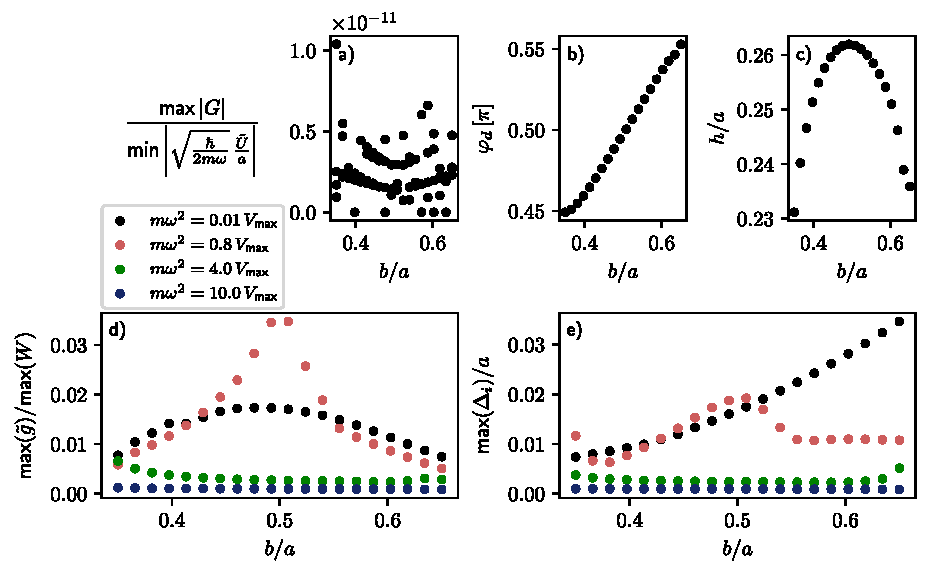
\includegraphics{pictures/tuning_first_order_to_zero4.pdf}
    \caption{\textbf{Parameters for negligible first order.} For different values of $m\omega^2$ the parameters $h$ and $\varphi_d$ are tuned such that the first order is negligible. The color code indicates the value of $m\omega^2/V_\text{max}$. The resulting ratio between first and second order is shown in panel a) for all considered values of $m\omega^2/V_\text{max}$ $0.01$, $0.8$, $4$ and $10$. As an example the optimal parameters $h$ and $\varphi_d$ for $m\omega^2/V_\text{max}=4$ are shown in panel b) and c). The maximal shift of the trap center necessary to eliminate the first order is shown in panel e), while panel d) shows that size of the shift is mainly determined by the ratio between $\tilde{g}$ and $W$. For the calculations a chain length of 8 atoms was used.}
    \label{fig:tuning_first_order_to_zero}
\end{figure}
% \hfill\newpage
\begin{figure}[h]
    \hspace*{-2cm}
    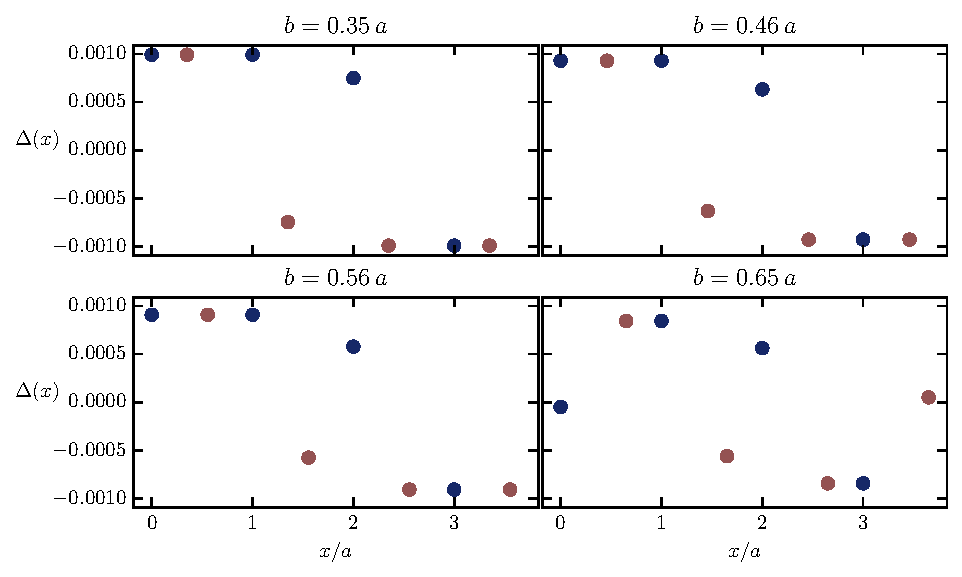
\includegraphics{pictures/Deltas4.pdf}
    \caption{\textbf{Trap center shift.} For $m\omega^2=10\,V_\text{max}$ the shift of the trap center for each site, that tunes the linear order to zero, is shown. The length of the chain is taken as 8 atoms.}
    \label{fig:tuning_first_order_to_zero_displacements}
\end{figure}
\figref{fig:tuning_first_order_to_zero} and \figref{fig:tuning_first_order_to_zero_displacements} tell us that the $\Delta$-displacements are of order $10^{-2}$, an order of magnitude bigger than the single motional mode displacement. Nevertheless the shift is small compared to the atomic distance $a$, which allows us to stick to the assumption of a periodic lattice. The shifts get smaller with increasing trap frequency. By eliminating the linear order, the Hamiltonian takes a quadratic form in the displacement and can hence be written as
\begin{align*}
    \mathcal{H}&=\sum_i\frac{\mathbf{P}_i}{2m} +\sum_i \frac12 m \omega^2 \,\delta\tilde{\mathbf{R}}_i^2  + \sum_{i,j}\delta\tilde{\mathbf{R}}_i\,U_{i,j}\,\delta\tilde{\mathbf{R}}_j 
\end{align*}
In second quantized from where I write the momentum and displacement operators in terms of creation and annihilation operators
\begin{align*}
    \delta\tilde{\mathbf{R}}_i &= \sqrt{\frac{\hbar}{2m\omega}}\,(a_i + a_i^\dagger)\\
    \mathbf{P}_i &= i\,\sqrt{\frac{\hbar m\omega}{2}}\,(a_i^\dagger - a_i)
\end{align*} 
the total Hamiltonian reads
\begin{align*}
    \mathcal{H} &= \sum_i \hbar\omega\,a_i^\dagger a_i +\frac{\hbar}{2m\omega}\, \sum_{i,j} U_{i,j}\,\left(a_i\,a_j + a_i^\dagger a_j + a_i\,a_j^\dagger + a_i^\dagger a_j^\dagger \right)\\
    &= \mathbf{a}^\dagger\,A\,\mathbf{a}
\end{align*}
with $\mathbf{a}=(a_1,\dots,a_N,a_1^\dagger,\dots,a_N^\dagger)$ the vector of operators and a coupling matrix $A$, which establishes the BdG form of the Hamiltonian and has itself the following structure
\begin{align*}
    A &= \frac{\hbar}{2m\omega}\,\begin{pmatrix}
       \bar{U} & U \\
       U & \bar{U}
    \end{pmatrix}\\
    \text{with}\quad \bar{U}&= U+m\omega^2.
\end{align*}
% This allows for a topological characterization of the bosonic system, acording to \cite{peanoTopologicalEdgeStates2018}. A first step is to consider the Heisenberg equations of motion for the operators which read %In order to understand the significance of the constant shift, one has to take into account the physical properties of the system. The Rydberg atoms, which have lifetimes up to $\sim200\,\mu$s, are trapped in optical tweezers of trap frequency up to $\sim2\,$MHz. This implies that one has to implement an Hamiltonian that induces non-trivial dynamics within the lifetimes of the atoms. Responsible for non-trivial dynamics is the U-matrix. Thus the interaction strength has to be at least as big as the trap frequency, i.e. $|U|\geq m\omega^2$. 


% \begin{align*}
%     \frac{d}{dt}\,{a}_j &= i\,([H,{a}_j]) = -i\, \hbar\omega a_j - i\,\frac{\hbar}{2m\omega}\,\sum_n \left(U_{j,n}\,a_n + U_{n,j}\,a_n + U_{j,n}\,a_n^\dagger + U_{n,j}\,a_n^\dagger\right) \\
%     &= -i\, \hbar\omega a_j -i\,\frac{\hbar}{m\omega}\,\sum_n \left(U_{j,n}\,a_n + U_{j,n}\,a_n^\dagger \right) = -2\,i\,(A\,\vec{a})_j\\
%     %
%     \frac{d}{dt}\,{a}^\dagger_j &= i\,([H,{a}^\dagger_j]) = i\, \hbar\omega a_j^\dagger  +i\,\frac{\hbar}{2m\omega}\,\sum_n \left(U_{j,n}\,a_n + U_{n,j}\,a_n + U_{j,n}\,a_n^\dagger + U_{n,j}\,a_n^\dagger\right) \\
%     &=  2\,i\,(A\,\vec{a})_{j+N}\\
% \end{align*}
% This lets one write the equations of motion in a different form
The dynamical matrix is then given by
\begin{align*}
    % \Rightarrow\quad \frac{d}{dt}\,\vec{a} &= -i\, H \,\vec{a}\\
    % \text{where}\quad 
   {H} &= \frac{\hbar}{m\omega}\,\begin{pmatrix}
       \bar{U} & U \\
       -U & -\bar{U}
       \end{pmatrix}
    %    =\vcentcolon \begin{pmatrix}
    %     h & \Delta\\
    %     -\Delta & -h
    %    \end{pmatrix}
\end{align*}
As it is a real matrix, it is time reversal symmetric. Particle-hole symmetry is also fulfilled, as $ \overline{H}=-\Sigma_x\, H \,\Sigma_x$ with 
\begin{align*}\Sigma_x=\begin{pmatrix}
    0 & \mathbb{1}\\
    \mathbb{1} & 0
\end{pmatrix}\end{align*}
Consequently it is then also chiral symmetric, as $ H =-\Sigma_x\, H \,\Sigma_x$. This puts the system in the BDI symmetry class, which allows for a topological characterization in one dimension. 
Since $H$ is not hermitian one has to investigate its spectrum for dynamical stability, i.e. no complex eigenenergies are allowed. \figref{fig:spectrum_BdG} shows that for small trapping depth compared to the phonon interactions always large imaginary contributions to the eigenvalues are observed. But for large tweezer strength ($m\omega^2=10\,V_\text{max}$), the imaginary part of the spectrum vanishes and also eigenstates inside of a gap are visible. %This motivates the computation of the system's winding number.
\begin{figure}[h]
    \hspace*{-2cm}
    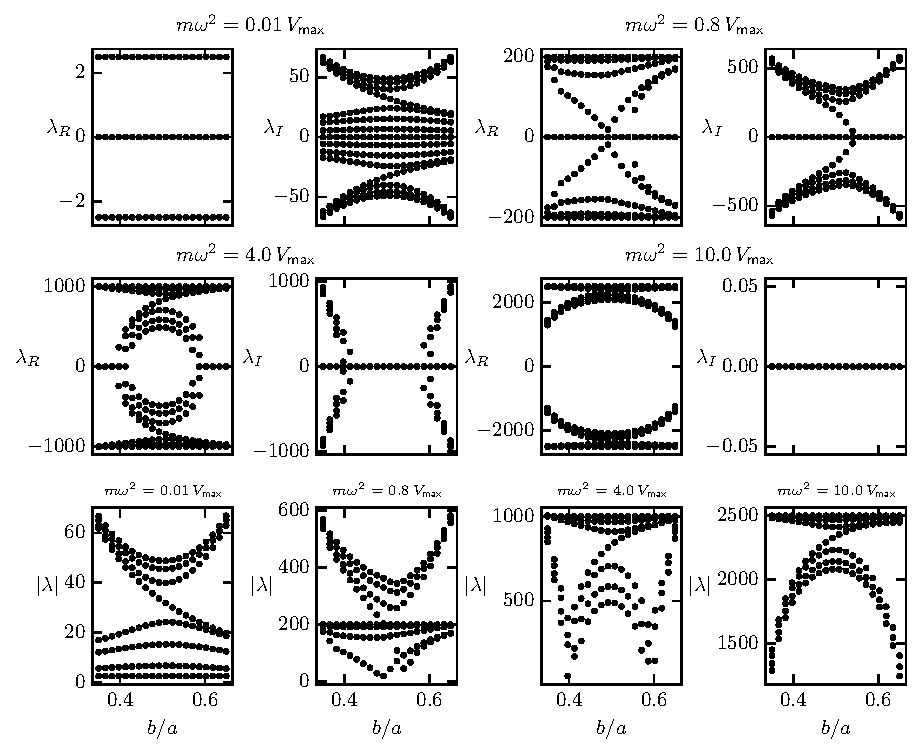
\includegraphics{pictures/spectrum_abs_of_tuned_BdG_various_shift_opt.pdf}
    \caption{\textbf{Spectrum of BdG Hamiltonian for different trap frequencies.} For different strengths of the optical trap the real and imaginary part of the spectrum is plotted. The atom number used for this computation is 8. In the last row the absolute value of the spectra is shown.}
    \label{fig:spectrum_BdG}
\end{figure}%\hfill\newpage
However by calculating the positive spectrum for larger atom numbers, as depicted in \figref{fig:pos_spectrum_different_chainlengths} one realizes that there is no real gap that withstands an infinite lattice size limit. This indicates that the system does not possess topological states, which can be affirmed by calculating the system's winding number, under the approximation that the periodicity breaking due to the small shifts of the trap center can be neglected.
\begin{figure}[h]
    \hspace*{-2cm}
    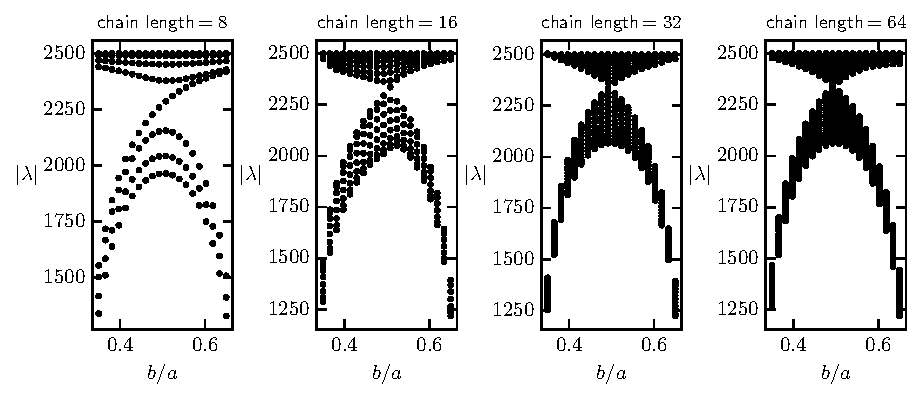
\includegraphics{pictures/spectrum_abs_of_tuned_BdG_various_chainlengths_for_gap_10V.pdf}
    \caption{\textbf{Positive spectrum of BdG Hamiltonian for different atom numbers.}}
    \label{fig:pos_spectrum_different_chainlengths}
\end{figure}

The first step is to transform the dynamical matrix into momentum space. When recapitulating the momentum space form of the general Bogoliubov-de Gennes Hamiltonian, \eqref{eq:Fourier Hamiltonian}, one can infer the structure of the dynamical matrix as
\begin{align*}
   H_k&=\begin{pmatrix}
        \tilde{U}(k) & U(k)\\
       - \overline{U(-k) }& -\overline{\tilde{U}(-k)}
    \end{pmatrix} =\begin{pmatrix}
        \tilde{U}(k) & U(k)\\
       - {U(k) }& -{\tilde{U}(k)}
    \end{pmatrix} 
\end{align*}
This form is independent of the explicit shape of $U$ and the potential. By assuming only that $U$ is generated by a second order expansion of a potential with two sublattices, i.e. \eqref{eq:U-matrix}, the form of $H_k$ can be inferred.
\begin{gather*}
    H_k = \begin{pmatrix}
        \tilde{U}(k) & U(k)\\
       - {U(k) }& -{\tilde{U}(k)}
    \end{pmatrix} \\
    \tilde{U}_k = \begin{pmatrix}
        b(k) & d(k)\\
        \bar{d}(k)& b(k)
    \end{pmatrix}\quad U_k = \begin{pmatrix}
        c(k) & d(k)\\
        \bar{d}(k) & c(k)
    \end{pmatrix}
\end{gather*}
Exploiting the symmetric structure of the matrix one can write
\begin{align*}
    H_k &= \tau_z \otimes \tilde{U}_k + i\tau_y \otimes U_k\\
    \tilde{U}_k &=  \sigma_0\,b(k)  + \sigma_x\,\text{Re}[d(k)] -\sigma_y\,\text{Im}[d(k)]\\
    U_k &=  \sigma_0\,c(k)  + \sigma_x\,\text{Re}[d(k)] -\sigma_y\,\text{Im}[d(k)]\\
    \Rightarrow\quad H_k &= b(k)\,\tau_z \otimes \sigma_0 + c(k)\,i\tau_y \otimes \sigma_0 + \text{Re}[d(k)]\,(\tau_z+i\tau_y) \otimes \sigma_x - \text{Im}[d(k)]\,(\tau_z+i\tau_y) \otimes \sigma_y
\end{align*}
where $\tau_\alpha$, $\sigma_\alpha$ $\alpha\in\{0,x,y,z\}$ are the usual Pauli matrices. In these expressions $b$, $c$, $d$ can be matrices treating the different directions of displacements from the trap center. The tensor product is not written explicitly in these cases.
Writing an arbitrary matrix in the form
\begin{align*}
    X&= \mathbb{1}\otimes A + \tau_x \otimes B + \tau_y \otimes C + \tau_z \otimes D
\end{align*}
one can compute the commutation relation by using
\begin{align*}
    \left[ O\otimes P, R\otimes S \right]&=\half \,[O,R]\otimes \{P,S\}+ \half\,\{O,P\}\otimes [R,S]
\end{align*}
\begin{align*}
    [H_k,X]&= \left[\left( \tau_z \otimes \tilde{U} + i \tau_y\otimes U\right)\;,\; \left(\mathbb{1} \otimes A + \tau_x \otimes B + \tau_y \otimes C + \tau_z \otimes D \right)\right] \\
&= \tau_z \otimes [\tilde{U}, A] + i \tau_y \otimes [U, A] + i \tau_y \otimes \{\tilde{U}, B\} + \tau_z \otimes \{U, B\} \\
&\quad - i \tau_x \otimes \{\tilde{U}, C\} + i \mathbb{1} \otimes [U, C] + \mathbb{1} \otimes [\tilde{U}, D] - \tau_x \otimes \{U, D\} \\
&= \mathbb{1} \otimes ( i[U, C] + [\tilde{U}, D] ) - \tau_x \otimes ( i\{\tilde{U}, C\} + \{U, D\} ) \\
&\quad + \tau_y \otimes ( i[U, A] + i\{\tilde{U}, B\} ) + \tau_z \otimes ( [\tilde{U}, A] + \{U, B\} )
\end{align*}
All of the summands are independent of each other, as are the pauli matrices. Therefore every summand has to vanish itself. To show that this is true I use the similarity of $\tilde{U}$ and $U$, in the form $\tilde{U}=\mathbb{1}\otimes b(k)+W$ and $U=\mathbb{1}\otimes c(k)+W$. The vanishing of the terms that come with $\mathbb{1}$ and $\tau_x$ yields 
\begin{align*}
    i\,[U,C] + [\tilde{U},D]&=0\\
    \Rightarrow\quad i\,[\mathbb{1}\otimes c(k),C]+ [\mathbb{1}\otimes b(k),D]+ [W,i\,C+D]&=0\\
    \text{and}\quad i\,\{\tilde{U}, C\} + \{U, D\}&=0\\
    \Rightarrow\quad i\,\{\mathbb{1}\otimes c(k),C\}+ \{\mathbb{1}\otimes b(k),D\}+\{W,i\,C+D\}&=0
\end{align*}
$b(k)$ and $c(k)$ differ only by a constant diagonal term, originating from the trap potential. This lets the last row read
\begin{align*}
    i\,\frac{\omega}{2}\,\{\mathbb{1},C\}+ \{\mathbb{1}\otimes b(k),i\,C+D\}+\{W,i\,C+D\}&=0
\end{align*}
By exploiting that this equation has to hold for any $k$ with $X$ $k$-independent and realizing that $b(k)$ and $W(k)$ are independent functions one follows that $C=0$ and therefore also $D=0$. Similarly one proceeds for the first and second term
\begin{align*}
    [U, A] + \{\tilde{U}, B\}&=0\\
    \Rightarrow\quad[\mathbb{1}\otimes c(k),A]+ \{\mathbb{1}\otimes b(k),B\}+[W,A]+\{W,B\}&=0\\
    [\tilde{U}, A] + \{U, B\}&=0\\
    \Rightarrow\quad[\mathbb{1}\otimes b(k),A]+ \{\mathbb{1}\otimes c(k),B\}+[W,A]+\{W,B\}&=0\\
    \Rightarrow\quad-\frac{\omega}{2}\,[\mathbb{1},A]+\frac{\omega}{2}\,\{\mathbb{1},B\}&=0\\
    \Rightarrow\quad B&=0
\end{align*}
Using again the independence of $b(k)$ and $W(k)$ one follows $[W,A]=0$. The matrix $W$ can then be written as
\begin{align*}
    W &= \sum_{\alpha,\beta\in\{0,x,y,z\}}w_{\alpha,\beta}(k)\,\sigma_\alpha\otimes\sigma_\beta\\
    &= \sigma_x\otimes\left( w_{x,0}\,\mathbb{1}+w_{x,x}\,\sigma_x+w_{x,z}\,\sigma_z \right)+\sigma_y\otimes\left( w_{y,0}\,\mathbb{1}+w_{y,x}\,\sigma_x+w_{y,z}\,\sigma_z \right)
\end{align*}
Due to the independence of the $w_{\alpha,\beta}(k)$ functions, $A$ has to commute with every summand individually. The only matrix which is not proportional to the identity, that commutes with the $\sigma_x$-term is $\sigma_x\otimes\mathbb{1}$. But this does not commute with the $\sigma_y$-term. Hence the $A$ has to be proportional to the identity and therefore $X$ has to be proportional to the identity.



% Combining the second and fourth row results in
% \begin{align*}
%     i\,C\,b(k)+D\,c(k)+W\,(i\,C+D)=0
% \end{align*}
% At this point it can be exploited that in order for X to be a symmetry of the system it has to commute with $H_k$ for all $k$ and hence be independent of $k$. Thus one can derive the equation by $k$ and can use $b'(k)=c'(k)$.
% \begin{align*}
%     (2\,b'(k)+W')\,(i\,C+D)=0
% \end{align*}
% This implies either $i\,C+D=0$ or $\text{Image}(i\,C+D)\subseteq \text{Kernel}(2\,b'(k)+W')$. In both cases there have to be vectors $\alpha\neq0$ such that
% \begin{align*}
%     (i\,C+D)\,\alpha=0\\
%     \Rightarrow\quad D\alpha=-i\,C\alpha
% \end{align*}
% Since every $4\times4$ matrix $X$ can be written in the form
% \begin{align*}
%     X = \sum_{\alpha,\beta\in\{0,x,y,z\}}x_{\alpha,\beta}\, \tau_\alpha \otimes \sigma_\beta
% \end{align*}
% one can conclude that the only matrix commuting with $H_k$ is the identity, i.e $[X,H_k]=0$ $\Rightarrow X=\mathbb{1}$. As no two different pauli matrices commute, the occurrence of $\tau_z$ and $\tau_y$ implies $x_{\alpha,\beta}=0$ for $\alpha\neq0$, similarly the occurrence of $\sigma_x$ and $\sigma_y$ implies $x_{\alpha,\beta}=0$ for $\beta\neq0$. 
Thus $H_k$ is irreducible as it has no unitary symmetries. This allows to perform a topological classification. %It is worth to mention that in the general form it can even be assumed that $b(k)$, $c(k)$ and $d(k)$ are symmetric matrices which couple modes of different directional displacement $x$, $y$, $z$. It has to be, however, assumed that these matrices are irreducible. With this requirement the irreducibility of the dynamical matrix remains intact. 
Exploiting the chiral symmetry, one can change to a basis where the chiral transformation $\Sigma_x^k=(\mathbb{1},-\mathbb{1})$. In this basis $H_k$ takes the form
\begin{gather*}
    H_k' = \begin{pmatrix}
        0 & S_k\\
        T_k & 0
    \end{pmatrix}= \half\,\begin{pmatrix}
        \mathbb{1} & \mathbb{1}\\
        \mathbb{1} & -\mathbb{1}
    \end{pmatrix}\,H_k\,\begin{pmatrix}
        \mathbb{1} & \mathbb{1}\\
        \mathbb{1} & -\mathbb{1}
    \end{pmatrix}\\\
    S_k = \begin{pmatrix}
        b(k)-c(k) & 0\\
        0 & b(k)-c(k)
    \end{pmatrix}\quad T_k = \begin{pmatrix}
        b(k)+c(k) & 2\,d(k)\\
        2\,\bar{d}(k) & b(k) + c(k)
    \end{pmatrix}
\end{gather*}% This is confirmed when looking at the eigenstates inside the gap of \figref{fig:spectrum_BdG}, when $m\omega^2=10\,V_\text{max}$.
As both matrices $S_k$ and $T_k$ are hermitian the Hamiltonian has vanishing winding number, indicating a topological trivial phase. The structure of $S_k$ and $T_k$ remains the same for higher dimensional displacements. I want to mention that if there are no pairing terms, i.e. $\mathbf{\Delta}=0$, the Hamiltonian is block diagonal and therefore not irreducible. In this case the introduction of holes is redundant and the winding number can be calculated from a single block, which can lead to non-vanishing winding numbers. It is thereby shown that the pairing terms prohibit the occurrence of topologically non-trivial phases in 1D for motional degrees of freedom stemming from a second order tailor expansion of an interaction potential.\hfill\newpage


\section{Excitation conservation}
In this section I want to discuss the case, where the trapping strength dominates over the the interaction between the atoms, i.e. $m\omega^2>>\text{max}(U)$. In this regime the creation of additional excitations through the interaction channel is suppressed and can be neglected. As a consequence the Hamiltonian can be projected onto a subspace of fixed excitation number, which is equivalent to a first order Schrieffer-Wolff transform. The result is that the terms that change the motional excitation number vanish and the Hamiltonian takes the form
\begin{align*}
    \mathcal{H}' &= \sum_i \hbar\omega\,a_i^\dagger a_i +\frac{\hbar}{2m\omega}\, \sum_{i,j} U_{i,j}\,\left( a_i^\dagger a_j + a_i\,a_j^\dagger  \right)
\end{align*}
By going into the reference frame of the harmonic trap oscillation, one can avoid the first term of this expression. The corresponding transform via $\exp(-it\omega\sum_ia_i^\dagger a_i)$ lets the Hamiltonian read
\begin{align*}
    \mathcal{H}&=\frac{\hbar}{m\omega}\, \sum_{i,j} U_{i,j}\,a_i^\dagger a_j\\
    &= (\mathbf{a}^\dagger)^t\,H\,\mathbf{a}\qquad\text{with }H=\frac{\hbar}{m\omega}\,\left(  U_{i,j} \right)_{i,j}
\end{align*}
Again the vector of annihilation operators is introduced $\mathbf{a}=(a_1,a_2,\dots)$, this time for the particle space only. The transformation into momentum space can also be performed in the annihilation/creation operator picture by dividing the system into two sublattices $L_A=(\mathbf{R}_1,\mathbf{R}_3,\mathbf{R}_5,\dots)$ and $L_B=(\mathbf{R}_2,\mathbf{R}_4,\dots)$. The operators in $A$ and $B$ transform via
\begin{align*}
    a_{\mathbf{k}} = \sum_{\mathbf{R}\in L_{A}} e^{-i\mathbf{k}\cdot\mathbf{R}}\,a_{\mathbf{R}}\\
    b_{\mathbf{k}} = \sum_{\mathbf{R}\in L_{B}} e^{-i\mathbf{k}\cdot\mathbf{R}}\,a_{\mathbf{R}}
\end{align*}
From this the Hamiltonian can be written in momentum space as well.
\begin{align*}
    \mathcal{H} &=\sum_{C,D\in\{A,B\}}\int_{\mathbb{T}^d}\frac{dk}{(2\pi)^d}\,\int_{\mathbb{T}^d}\frac{dk'}{(2\pi)^d}\,  \sum_{\substack{\mathbf{R}\in L_C;\,\mathbf{R}'\in L_D}}H(\mathbf{R}-\mathbf{R}')\,e^{-i\,(\mathbf{k}\mathbf{R}-\mathbf{k}'\mathbf{R}')}\, c_{\mathbf{k}}^{\dagger} d_{\mathbf{k}'}\\
    &=\sum_{C,D\in\{A,B\}}\int_{\mathbb{T}^d}\frac{dk}{(2\pi)^d}\,\int_{\mathbb{T}^d}\frac{dk'}{(2\pi)^d}\,  \sum_{\substack{\mathbf{R}\in L_C;\,\Delta\mathbf{R}\in\{ L_D-L_C\}}}H(\Delta\mathbf{R})\,e^{-i\,(\mathbf{k}-\mathbf{k}')\,\mathbf{R}+i\,\mathbf{k}'\Delta\mathbf{R}}\, c_{\mathbf{k}}^{\dagger} d_{\mathbf{k}'}\\
    &=\sum_{C,D\in\{A,B\}}\int_{\mathbb{T}^d}\frac{dk}{(2\pi)^d} \sum_{\substack{\Delta\mathbf{R}\in\{ L_D-L_C\}}}H(\Delta\mathbf{R})\,e^{i\,\mathbf{k}\Delta\mathbf{R}}\, c_{\mathbf{k}}^{\dagger} d_{\mathbf{k}}\\
    &=:\int_{\mathbb{T}^d}\frac{dk}{(2\pi)^d}\sum_{C,D\in\{A,B\}} H_\mathbf{k}^{C,D}\, c_{\mathbf{k}}^{\dagger} d_{\mathbf{k}}=:\int_{\mathbb{T}^d}\frac{dk}{(2\pi)^d}\, (\mathbf{a}_{\mathbf{k}}^\dagger)^t\,H_\mathbf{k}\,\mathbf{a}_{\mathbf{k}}
\end{align*}
with $\mathbf{a}_\mathbf{k}=(a_\mathbf{k},b_\mathbf{k})$. 
Since $\Delta\mathbf{R}^{A,B}=-\Delta\mathbf{R}^{B,A}$ and $\Delta\mathbf{R}^{A,A}=\Delta\mathbf{R}^{B,B}$ the form of $H_\mathbf{k}$ is 
\begin{align}\label{eq:H_k decomposition}
    H_\mathbf{k}&=\begin{pmatrix}
        H_\mathbf{k}^{A,A} & H_\mathbf{k}^{A,B}\\
        (H_\mathbf{k}^{A,B})^* & H_\mathbf{k}^{A,A}
    \end{pmatrix}\notag\\
    &=\mathbb{1}\otimes H_\mathbf{k}^{A,A} + \sigma_x\otimes\text{Re}\left[ H_\mathbf{k}^{A,B} \right]-\sigma_y\otimes\text{Im}\left[ H_\mathbf{k}^{A,B} \right]
\end{align}
The submatrices of $H_\mathbf{k}$ can again be matrices themselves that couple the different directions of displacement and thus have the form of
\begin{align}\label{eq:xy-decomposition}
    O &= O_0\,\mathbb{1}+ O_x\,\sigma_x+ O_z\,\sigma_z
\end{align}
In this case the matrix $H_\mathbf{k}$ is only irreducible if it contains non-zero $\sigma_x$ and $\sigma_y$ contributions in the first slot of the tensor product as well as $\sigma_x$ and $\sigma_z$ contributions in its second slot.
It is important to note that the decomposition of $H_k$ into pauli matrices contains only independent functions of $k$ as coefficients.
\subsection{One dimensional chain}
As a one-dimensional chain I will investigate the zik-zak configuration with alternating distances, as depicted in \figref{fig:chain scheme}. Because the Hamiltonian derived in \secref{sec:model derivation} is $T=+1$ time reversal symmetric, with respect to the Altland-Zirnbauer symmetry classes \cite{ryuTopologicalInsulatorsSuperconductors2010}, the only possibility in 1D that lets the system possess topological phases requires the Hamiltonian to be in the BDI class and thus be particle-hole and chiral symmetric. With the knowledge of time reversal symmetry the latter to symmetries imply each other and it suffices to show that one of those symmetries is satisfied. For a $H_k$ to be chiral symmetric one demands, as stated in \secref{sec:winding number}, that $\{H_k,X\}=0$ for an unitary matrix $X$. 



% In the case with only one-dimensional displacements one immediately recognizes that chiral symmetry is only fulfilled if the term $H_k^{A,A}$ vanishes. This is only possible for all $k$ if the Hamiltonian does not couple sites within the same sublattice. 


\begin{figure}[h]
    % \hspace*{-2cm}
    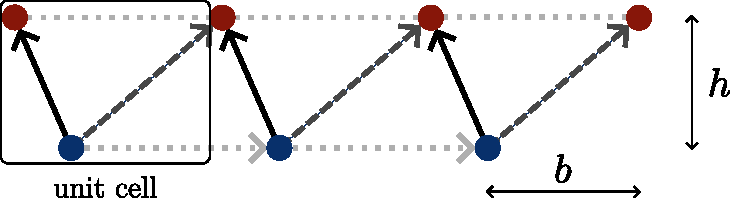
\includegraphics{pictures/chain_with_interaction_arrows_wo_dipole.pdf}
    \caption{\textbf{Zik-zak chain.} Interactions up to next nearest neighbors are presented. The two sublattices A and B are depicted in colors red and blue respectively.}
    \label{fig:chain scheme}
\end{figure}
The difference in trap depth with respect to the axial versus the radial direction of the trap allows to decouple axial ($z$-axis) and radial $xy$-plane degrees of freedom. If the difference in trap potential is much larger than the interactions between the motional degrees of freedom mediation between these two directions is suppressed. If additionally an elliptical shaped trap is realized where trapping strength in $x$ and $y$-direction differ by a significant amount, one can restrict oneself to the consideration of only one dimensional displacements, as all three directions decouple from each other.

For displacements only along the $x$-axis, $H_k^{A,A}$ and $H_k^{A,B}$ become just complex numbers. The only way that the system possesses chiral symmetry is then that $H_k^{A,A}=0$. This requires on the one hand that interactions between sublattices vanish and on the other hand the onsite terms of the interaction matrix. Interactions within one sublattice can be tuned to zero by choosing the $x$-component of the dipole unit-vector to $d_x=1/\sqrt{3}$. But the onsite terms are an inherent feature of the model stemming from the second order expansion of the dipole potential and cannot be avoided by the geometry of the system. These onsite terms destroy the chiral symmetry of the chain and prohibit edge-states to form. \figref{fig:1D dis edge occupation} shows what happens if the diagonal of matrix $U$ is artificially multiplied by a factor $\alpha\in[0,1]$. As the diagonal terms of $U$ are of the same magnitude as the other coupling strengths, the in-gap states get expelled from the gap and loose their edge-occupation as $\alpha$ is increased. $\alpha=1$ restores the original $U$ matrix and it is seen that no edge states prevail in this scenario.
\begin{figure}[H]
    % \hspace*{-2cm}
    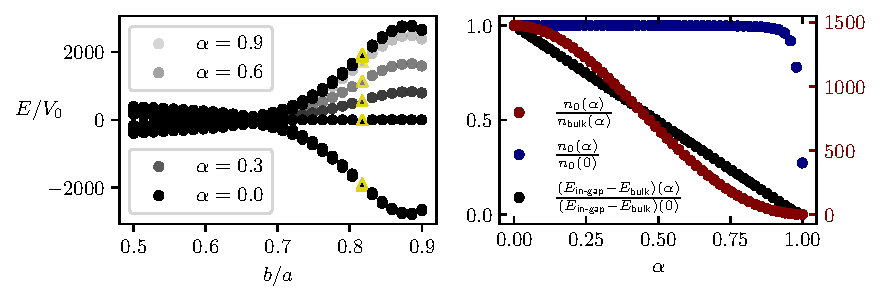
\includegraphics{pictures/edge_occupation_alpha2.pdf}
    \vspace*{-0.3cm}
    \caption{\textbf{Edge occupation in dependence of onsite potential strength.} The left panel shows the spectrum of $H$ in dependence of the spacing between the atoms for different values of $\alpha$. Energies are given in units of $V_0=\hbar V(a)/(2m\omega a^2)$. In the diagram, $\alpha$ is an artificial factor with whom the diagonal of matrix $H$ is multiplied, in order to show how this term pulls the in-gap modes into the bulk. For the highlighted $b$-values the left panel shows how the edge occupation degrades with increasing $\alpha$.}
    \label{fig:1D dis edge occupation}
\end{figure}

By tuning the trap potential in such a way that it compensates the inhomogeneity of the diagonal of $H$, one would restore the chiral symmetry and edge states of the system. The state of the art precision when it comes to the homogeneity of optical tweezer depth in an array lies around 2\% \cite{taoHighFidelityDetectionLargeScale2024}. According to \secref{sec:dipole traps} one can estimate the precision in overall trap frequency to be around 1\%. This ratio is also in the order of magnitude of the ratio between interaction and trapping frequency for the model at hand. It is therefore just at the edge of being able to reduce the onsite terms of the interaction matrix in an sufficient way, as to bring the boundary-localized in-gap modes back to the spectrum. Hence, at this current state the trap frequency can on its own be a source of uncertainty that brakes the edge localization of states, but future improvements in the precision of trap strength configuration could allow to tune the system to a proper topological phase.




For displacements along both $x$ and $y$-direction, where equal trap strength along both directions is assumed, the only way chiral symmetry can be meaningfully fulfilled is for vanishing $H_k^{A,A}$. This is however not achievable by any choice of geometry. It is only possible to realize an optimal configuration in form of the  distance between the sublattices together with the orientation of the dipole moment that lets $H_k^{A,A}$ be up to an order of magnitude smaller than the other coupling. The optimal ratio $H_k^{A,A}/H_k^{A,B}$ is shown in \figref{fig:optimal ratio AA to AB} for different lattice configurations.  It was also assumed that the onsite terms get cancelled by an appropriate choice of the trap potentials. 
\begin{figure}[h]
    \hspace*{-2cm}
    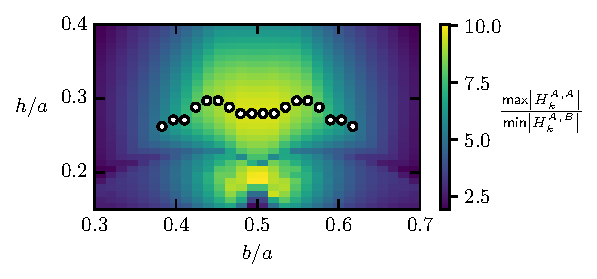
\includegraphics{pictures/optimal_tuning_HAA_vs_HAB.pdf}
    \caption{\textbf{Optimal ratio between maximum of $H_k^{A,A}$ and minimum of $H_k^{A,B}$.} The ratio is computed taking to account nearest neighbor interactions for $H_k^{A,B}$ and next to nearest neighbor interactions for $H_k^{A,A}$. The circles depict the 1D cross section for which the spectrum and the edge occupation is considered in \figref{fig:edge occupation 2d dis}. }
    \label{fig:optimal ratio AA to AB}
\end{figure}
The chiral symmetry is not satisfied for these configurations. But one can nevertheless analyze if there are states inside of the bulk gap that are well localized at the edges of the chain. This is shown in \figref{fig:edge occupation 2d dis}. One actually finds modes inside the bulk gap, which are localized at the edges, but neither lie the energies of these states perfectly in the middle of the gap at zero energy, nor are the states completely restricted to edge excitations. On the other hand one can find states inside the bulk spectrum which are orders of magnitude better localized. These states are however not protected by the bulk gap against perturbations.  
\begin{figure}[h]
    % \hspace*{-2cm}
    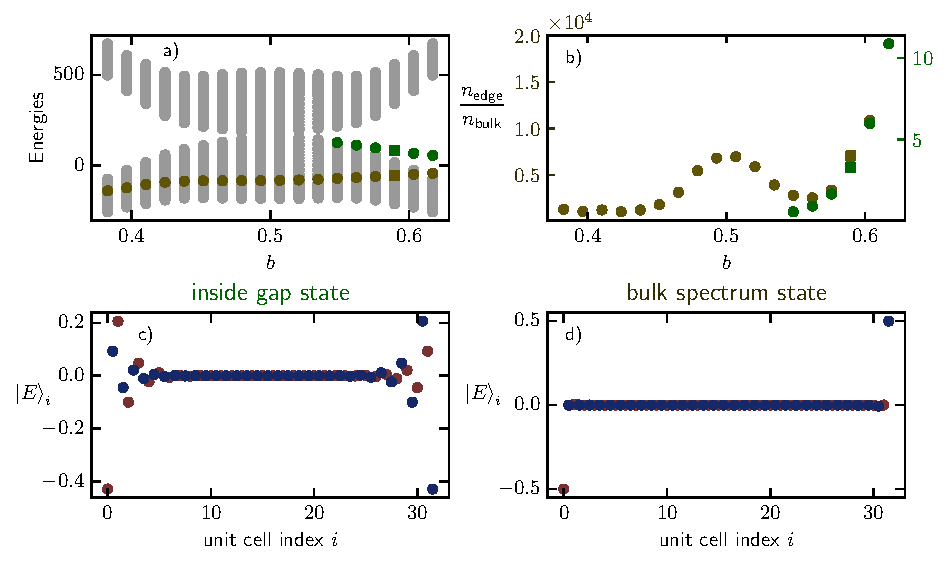
\includegraphics{pictures/edge_occupation_xy_model.pdf}
    \caption{\textbf{Spectrum and edge states for 2D displacement.} For the cross section specified in \figref{fig:optimal ratio AA to AB} the spectrum is presented in a). Inside the bulk gap as well as inside the bulk spectrum states are found that are highly localized at the boundaries of the system. These states are depicted in c) and d) respectively. Figure c) shows the ratio of edge occupation to bulk occupation, where the edge contains the outer four sites of the chain.}
    \label{fig:edge occupation 2d dis}
\end{figure}